\chapter{Megvalósítás}

\section{Grafikák elkészítése}

\indent \indent Mielőtt nekiláttam a grafikai elemek létrehozásának, inspirációként szolgáltak az interneten elérhető rajzolási stílusok és csempekészletek. Az alapja és mintája a saját rajzaimnak a Ninja Adventure Tileset volt, amelyet Pixel-boy készített.\cite{NAT}

\subsection{Grafikus szerkesztő}

\indent \indent Fontos kiemelni, hogy egy ``pixelart'' rajz stílusról beszélünk az esetemben, ezért kerestem olyan rajzprogramot, amely minden igényemet kielégíti és könnyen kezelhető tapasztalatlan grafikusok számára is. A kiválaszott program az Aseprite volt, ebben készítettem minden játékban megtalálható grafikát. (Lásd \ref{fig:Aseprite} ábra)

\begin{figure}[H]
    \centering
    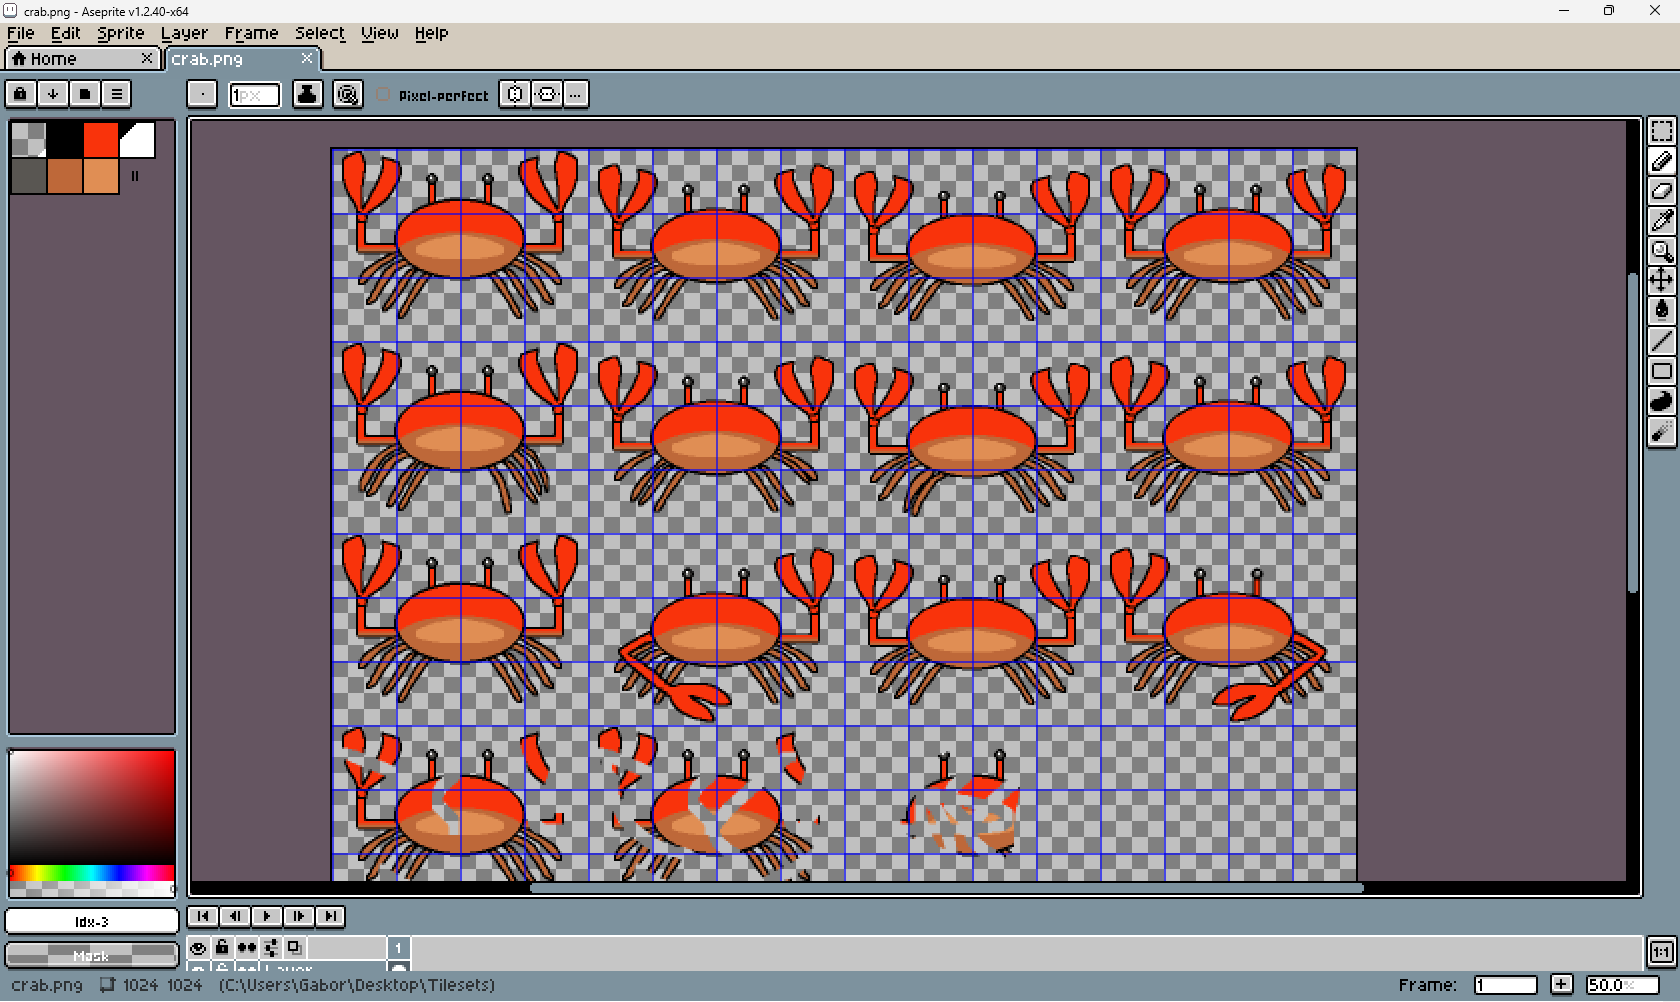
\includegraphics[width=14.0truecm]{images/Aseprite.png}
    \caption{Aseprite - Pixelart rajzoló program
    \cite{Aseprite}}

    \label{fig:Aseprite}
\end{figure}


\subsection{Rajzok elkészítése}

\indent \indent A rajzok elkészítése két fő részből állt, a pálya tervezéséből és a karakterek, valamint a környezet kialakításából. A pálya tervezéséhez a korábban említett Ninja Adventure Tileset szolgált mintaként, melyből az összes pálya elemét saját kezűleg rajzoltam meg. A karakterek és környezet rajzainak elkészítésénél pedig meglévő rajzokat használtam inspirációként, és ezeket egészítettem ki saját kreatív ötleteimmel.

\subsubsection{Pálya}
\indent \indent A pályaelemek létrehozásánál kiemelkedően fontos volt figyelnem arra, hogy a csempék harmonikusan illeszkedjenek egymáshoz, ezáltal kellemes és összefüggő látványt teremtve.

\begin{figure}[H]
    \centering
    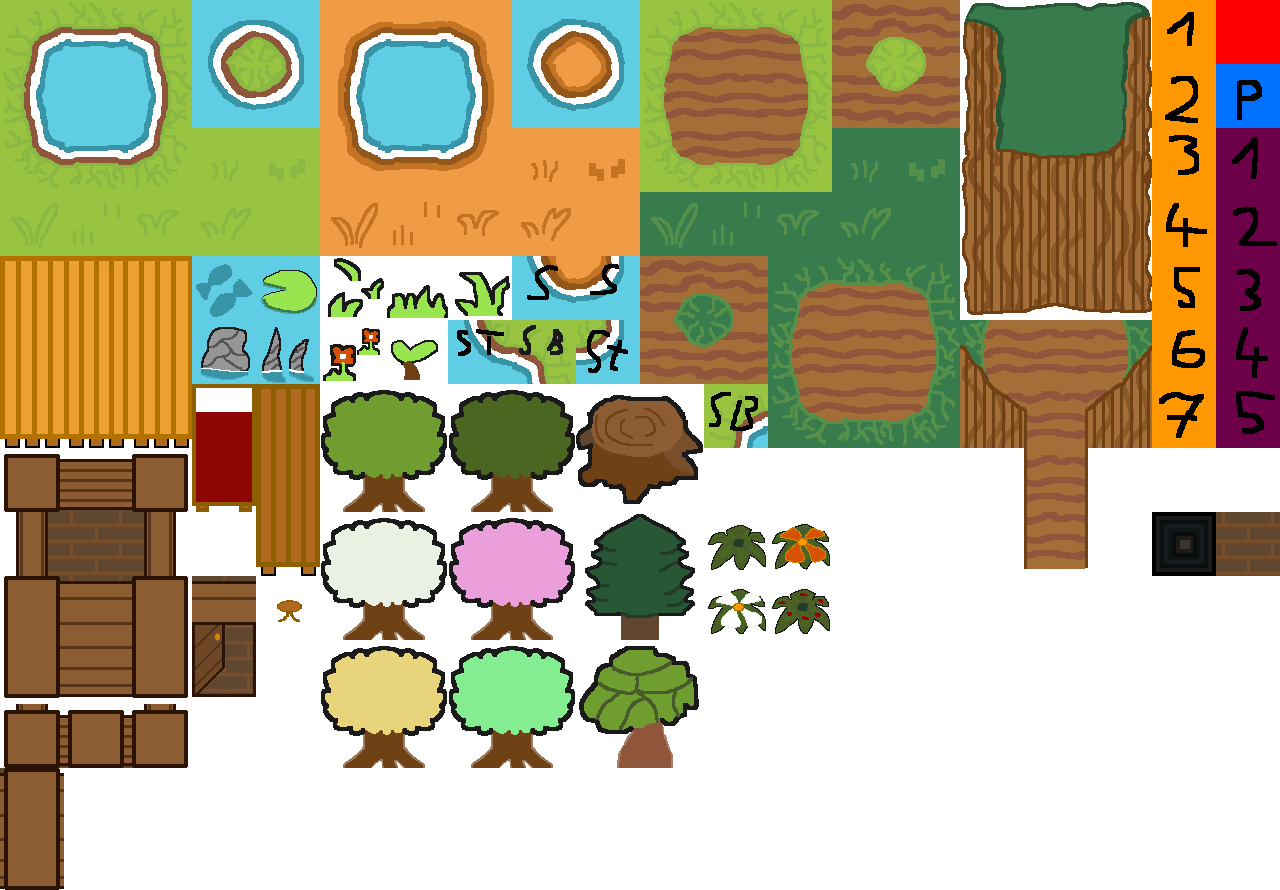
\includegraphics[width=12.0truecm]{images/tileset.png}
    \caption{Csempekészlet}
    \label{fig:Csempekészlet}
\end{figure}

\subsubsection{Entitások}
\indent \indent Karakterek és szörnyek megtervezése annyiban tért el, hogy ott figyelni kellett az animációra is, mert élethű mozgást szerettem volna utánozni. Egy ilyen mozgás animáció 4-6 képből áll, amelyeket egymás után lejátszva érhető el a kívánt hatás. Illetve, mivel 4 különböző irányba tudnak haladni ezek az entitások, ezért 4 különböző animációt kellett elkészítenem, amelyeket a játék során a karakter irányának megfelelően tudtam lejátszani, ez látható a \ref{fig:Aseprite} ábrán.

\begin{figure}[H]
    \centering
    
\includegraphics[width=12.0truecm]{images/entities.png}
    \caption{Entitások}
    \label{fig:Entitások}
\end{figure}


\section{Pálya megtervezése}

\subsection{Tiled}
\label{subsec:Tiled}
\indent \indent A pálya megtervezéséhez a Tiled-et \cite{Tiled} választottam, ami egy népszerű térképszerkesztő szoftver, amelyet játékfejlesztők használnak a 2D-s játékok pályáinak tervezésére és szerkesztésére.   A Tiled egy nyílt forráskódú program, így ingyenesen elérhető és széles körben használt az indie játékfejlesztők körében.

Ez a szoftver lehetővé teszi a felhasználók számára, hogy könnyen létrehozzanak és testreszabjanak térképeket, amelyeket különböző játékkeretrendszerekbe integrálhatnak. A Tiled számos funkciót kínál, mint például csempekészletek használata, rétegek kezelése, objektumok lehelyezése rácshálóra, ezzel elkerülve a rétegen belüli átfetéseket. (Lásd \ref{fig:Tiled} ábra) Valamint az exportálás különböző formátumokban, például CSV (Coma-Separated Values) vagy TMX (Tiled Map XML).

Az egyszerű és intuitív felhasználói felülete miatt amit a \ref{fig:Tiled}-es ábrán is lehet látni, a Tiled ideális eszköz a játékfejlesztők számára, akik az apró részletekre is figyelő térképeket szeretnének készíteni játékaikhoz. Az XML alapú TMX formátum kompatibilis a legtöbb játékmotorral, így a Tiled segítségével készült térképek könnyen beilleszthetők a fejlesztési folyamatba.

\begin{figure}[H]
    \centering
    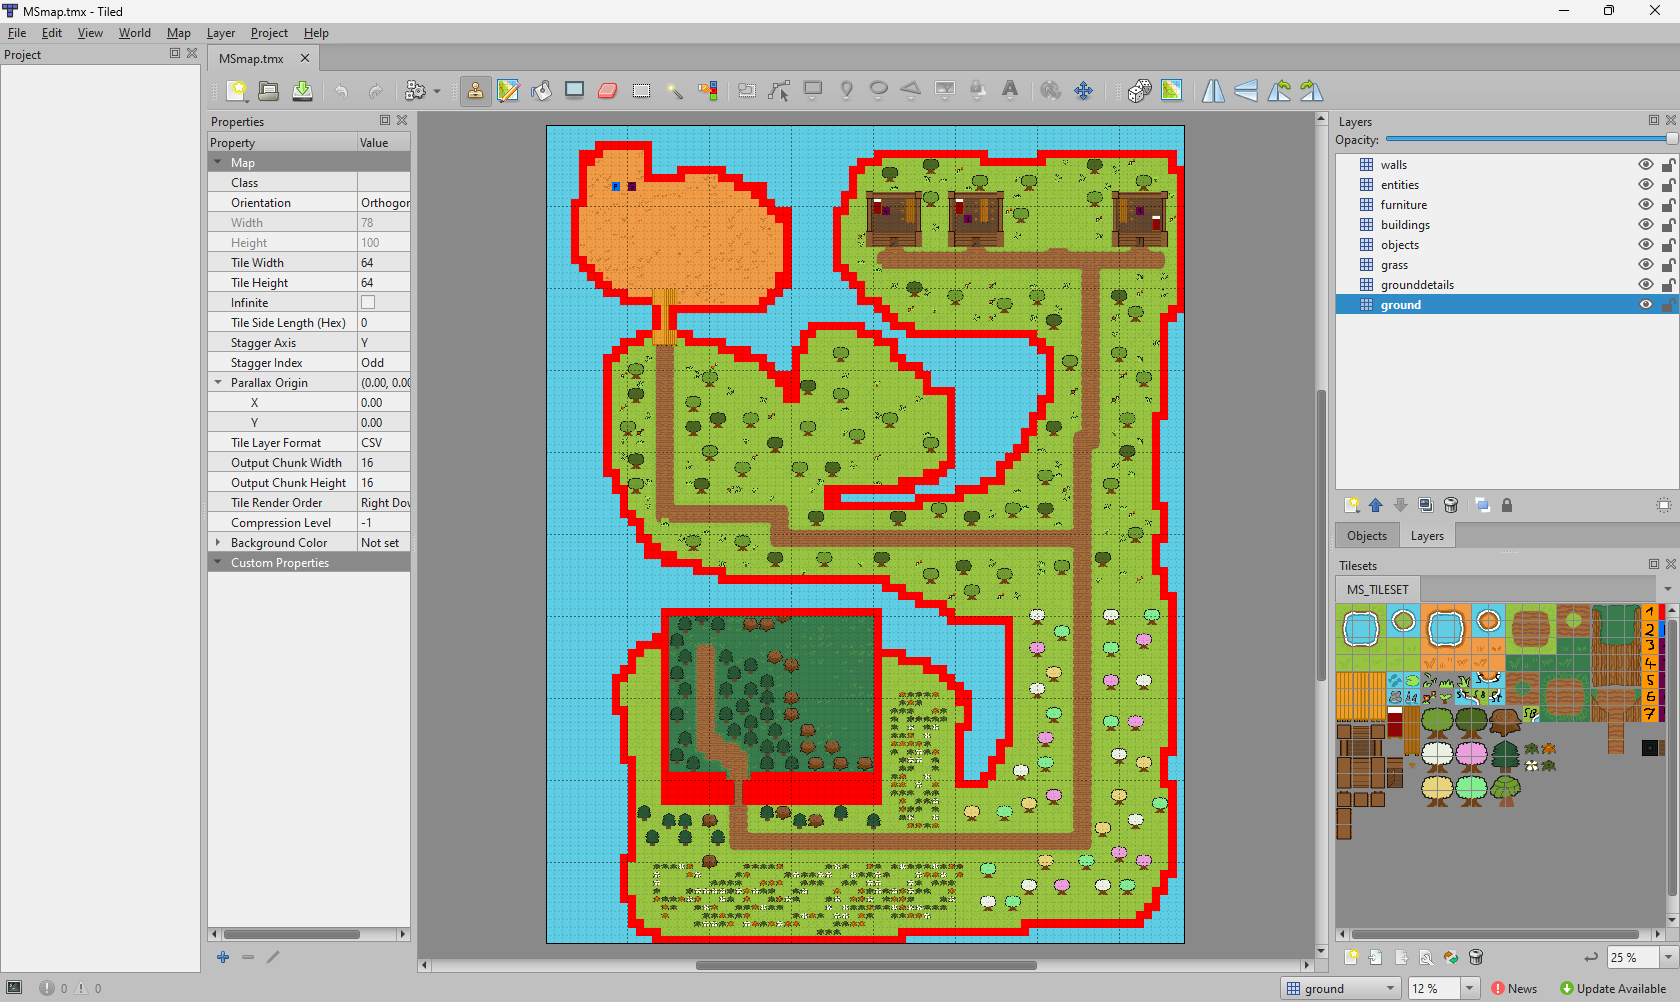
\includegraphics[width=14.0truecm]{images/Tiled.png}
    \caption{Tiled - Pálya szerkesztő
    \cite{Tiled}}
    \label{fig:Tiled}
\end{figure}

\subsection{Tervezés} \label{subsec:Tervezés}

\indent \indent Kiemelkedően fontos volt a pálya elemeit különböző rétegekre szétválasztani, ezáltal megkönnyítve a fejlesztést és az egyes részek kezelését. A háttér szolgálatában álló csempéket például két rétegre osztottam: az egyikre a talajszintet, a másikra pedig a talajon megtalálható növényzetet helyeztem el. Ezt a két réteget együttesen exportáltam PNG formátumban, amelyet a játékban háttérképként használtam. Fontos megjegyezni, hogy a két háttér réteget nem mentettem külön CSV fájlba. Ennek oka az, hogy ezek a rétegek olyan elemeket tartalmaznak, amelyek statikusak és nincs velük semmiféle interakció a játék során. 

Van még egy fontos réteg amik akadályként szolgálnak a játékos számára (Lásd \ref{fig:Tiled} ábra piroskörvonal), ezeket a rétegeket a játékos nem tudja átlépni, ezáltal a játékmenetet befolyásolják.  

További rétegek lettek létrehozva az objektumok számára, minden típusú objektumot külön rétegen helyeztem el, így könnyen kezelhetőek és nem kell a kódban szűrést alkalmazni a különböző típusú objektumok használatakor.
A következő elemeknek hoztam létre saját réteget: talajnak, talajon megjelenő részleteknek ez ahogy az előbb említettem össze tartoznak. A játék során kiüthető objektumoknak, jelenleg a fűcsomók. Nem kiüthető objektumoknak, például házak vagy fák. Berendezési tárgyaknak, mivel azokat talajként szerettem volna kezelni, de nem felülírva a hátteret. Falaknak az pályahatárok meghatározásához. Illetve nem utolsó sorban az entitásoknak, hogy milyen pozícióra rajzolja ki őket a játék.  (Lásd \ref{fig:Tiled} ábra)


% \section{Megvalósított rendszerek bemutatása}
% \indent \indent A következő szekcióban a játékban megvalósított rendszereket mutatom be, amelyek a játékmenetet és a felhasználói élményt szolgálják. A rendszerek részletes leírása mellett bemutatom a kód részleteket is, amelyek segítségével könnyen megérthető, hogyan történik az egyes rendszerek működése.

\section{Felhasználói felület és beállítások kezelése}

\subsection{Beállítások}
\indent \indent A funkció fő célja a beállítások kezelése egy játékban vagy alkalmazásban. Az osztály tartalmazza az alapértelmezett beállításokat, mint például a játékablak méretét, a hangerejét és egyebeket. Az osztály segítségével ezeket a beállításokat be lehet tölteni vagy menteni egy JSON fájlba.

Az ott statikus osztályváltozók az alapértelmezett értékeket tárolják, és a program különböző részeiben felhasználhatók, anélkül, hogy az osztalyt peldanyositani kellene, így könnyen hozzáférhetőek.

További adatokat is tartalmaz, például hangokat, grafikákat, karaktereket, ellenségeket, lövedékeket és fegyvereket. Mindezek az adatok részletezik a játékbeli objektumok tulajdonságait. Azért ezt a megoldást választottam, mert így könnyen kezelhetőek és könnyen módosíthatóak a játékbeli objektumok tulajdonságai. Egyhelyen kezelve egyszerűbb a karbantartás is, ha egy szörny túl erős lenne vagy egy fegyver túl gyenge, akkor csak egy helyen kell módosítani az adatokat, és az összes példányban azonnal érvényesülnek a változtatások.

Az osztály emellett definiálja a felhasználói felület színeit és stílusait, amelyek a játék megjelenítéséhez használok. Ez azért fontos, hogy egységes megjelenést biztosítson a felhasználói felületben, és ahogy az előbb is említettem, egy színkód megváltoztatásával mindenhol azonnal érvényesül a változtatás.


\subsection{Felhasználói fiók}
\indent \indent Ez a rendszer kezeli a regisztrációhoz és a bejelentkezéshez kapcsolódó folyamatokat. Ilyen folyamat többek között a felhasználói felület megjelenítése, de a tartalomellenőrzés és hibakezelés is. Tartalomellenőrzés alatt a felhasználónév és jelszó validálás értendő, hogy megfelelő formátumban vannak-e megadva. Hibakezelés alatt pedig a felhasználó értesítése, ha valamilyen hiba történik a regisztráció vagy bejelentkezés során. regisztráció esetén, ha sikeres validálás történik, akkor md5 hash algoritmus segítségével titkosítva tárolja a jelszót az adatbázisban. Bejelentkezéskor ezt a titkosított jelszót hasonlítja össze a felhasználó által megadott jelszó titkosított formájával, ha megegyezik, akkor engedi a bejelentkezést.

\subsection{Főmenü}

\indent \indent A játéknak elengedhetetlen része a főmenü, ami a bejelentkezés után válik elérhetővé a felhasználók számára. Biztosítok a játékosoknak offline, azaz internet nélküli játszási lehetőséget, ilyenkor regisztráció és bejelentkezés nélkül használni lehet a játékot.
A főmenüben legfelül a játék címe ``Marooned Sailor'' jelenik meg, alatta három menüpont található meg, az új játék létrehozása, meglévő mentés betöltése, illetve a beállítások. Kijelentkezési lehetőséget nem valósítottam meg, ahogy kilépés gombot sem helyeztem el, ezzel szeretném ösztönözni azokat akik kipróbálják, hogy ne zárják be első látásra a játékot. Bezárni az asztali alkalmazást a pillanat állj menüben lehet majd a játék során az exit menüpontra kattintva. (Lásd \ref{fig:Főmenü} ábra) 

\begin{figure}[hbt]
    \centering
    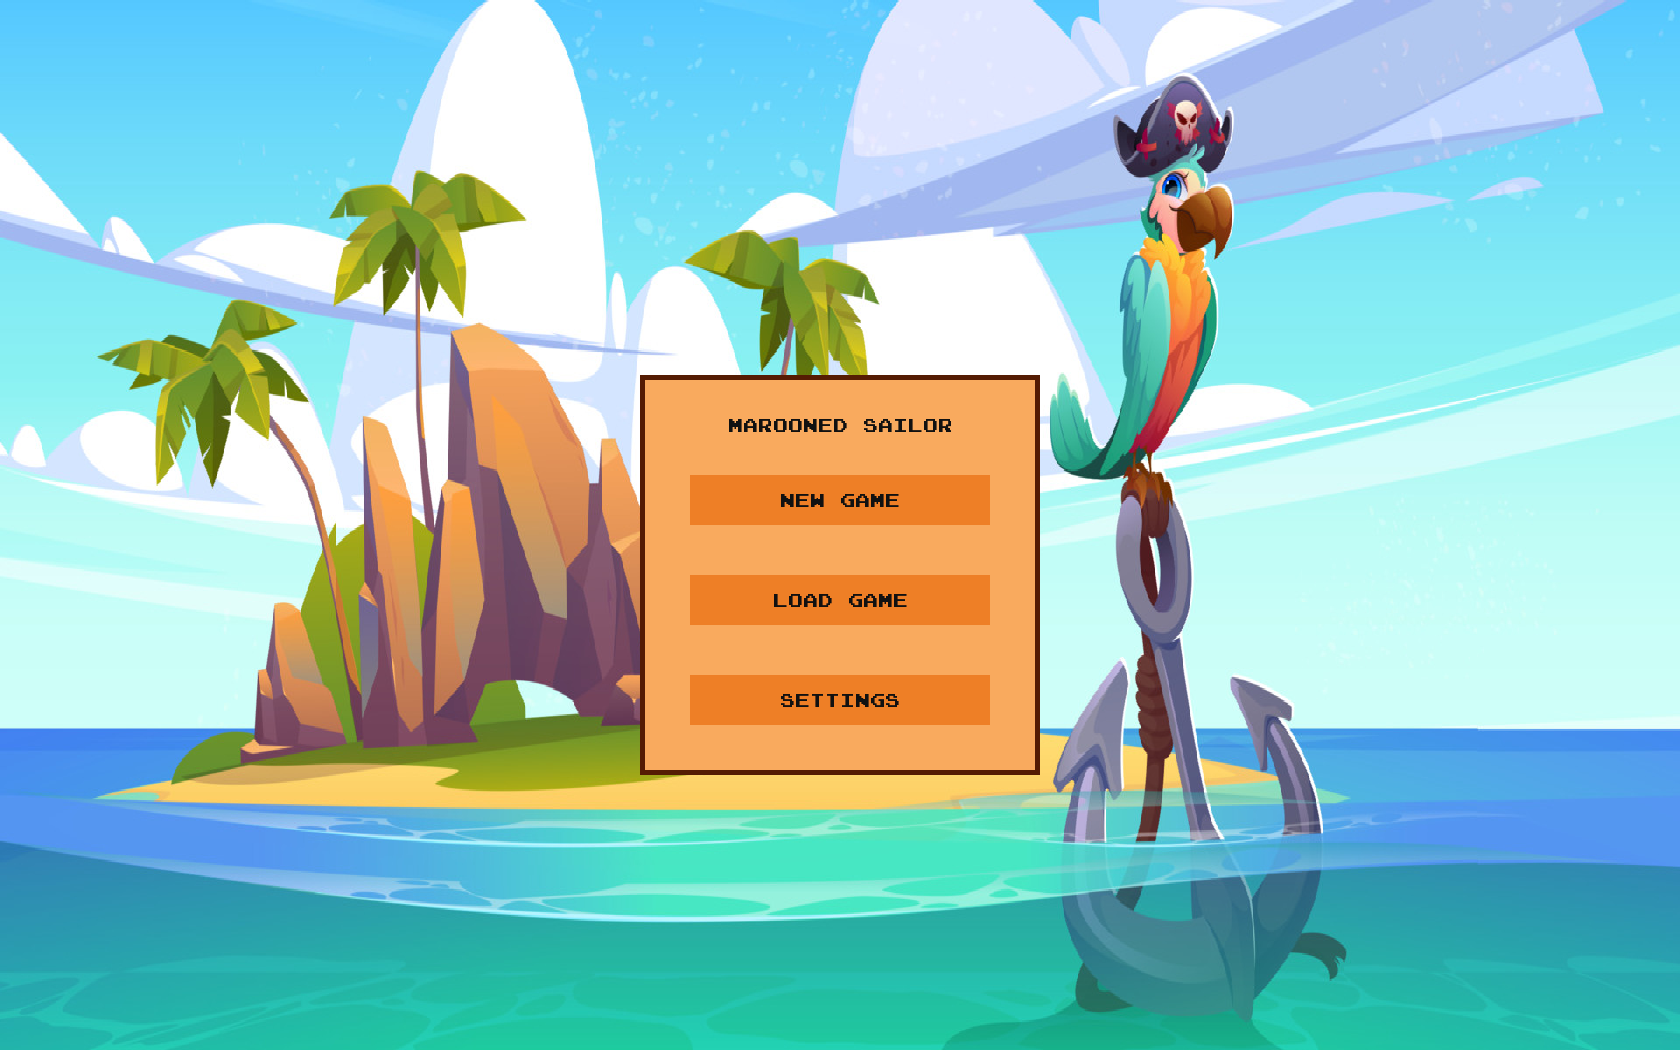
\includegraphics[width=14.0truecm]{images/mainmenu.png}
    \caption{Főmenü}
    \label{fig:Főmenü}
\end{figure}


\subsection{Új játék létrehozása}
\indent \indent Az új játék menüpont kiválasztása után (lásd \ref{fig:Új játék létrehozása}) a játékosnak meg kell adni a karakterének a nevét, illetve választhat különböző karakter kinézetek közül. Ha be van jelentkezve a játékos, akkor van lehetősége nehézségi szintet is választani.
A nehézségi szint annyiban különbözik, hogy a ``normal'' módban, ha elfogynak a játékos életpontjai, akkor a játék folytatódik tovább, újraéled egy bizonyos helyen. Viszont, ha a ``challange'' (kihívás) módot választja, akkor három funkcióval bővül a játékmenet. Az első ilyen funkció, hogy ha elfogy a játékos életereje, akkor véglegesen meghal a karakter, és nem lesz lehetősége tovább folytatni azzal a bizonyos karakterrel a játékot. A második plusz funkció, hogy az összes küldetés teljesítése esetén a játék újrakezdődik, amely azt eredményezi, hogy a szörnyek erősödnek, és nagyobb kihívás lesz újra végigvinni az összes küldetést. Illetve tartalmaz egy ranglista menüpontot, amely jelzi a legügyesebb játékosok hányszor tudták a ``challange'' mód használatával végigvinni az összes küldetést. (Lásd \ref{fig:Új játék létrehozása} ábra)

\begin{figure}[H]
    \centering
    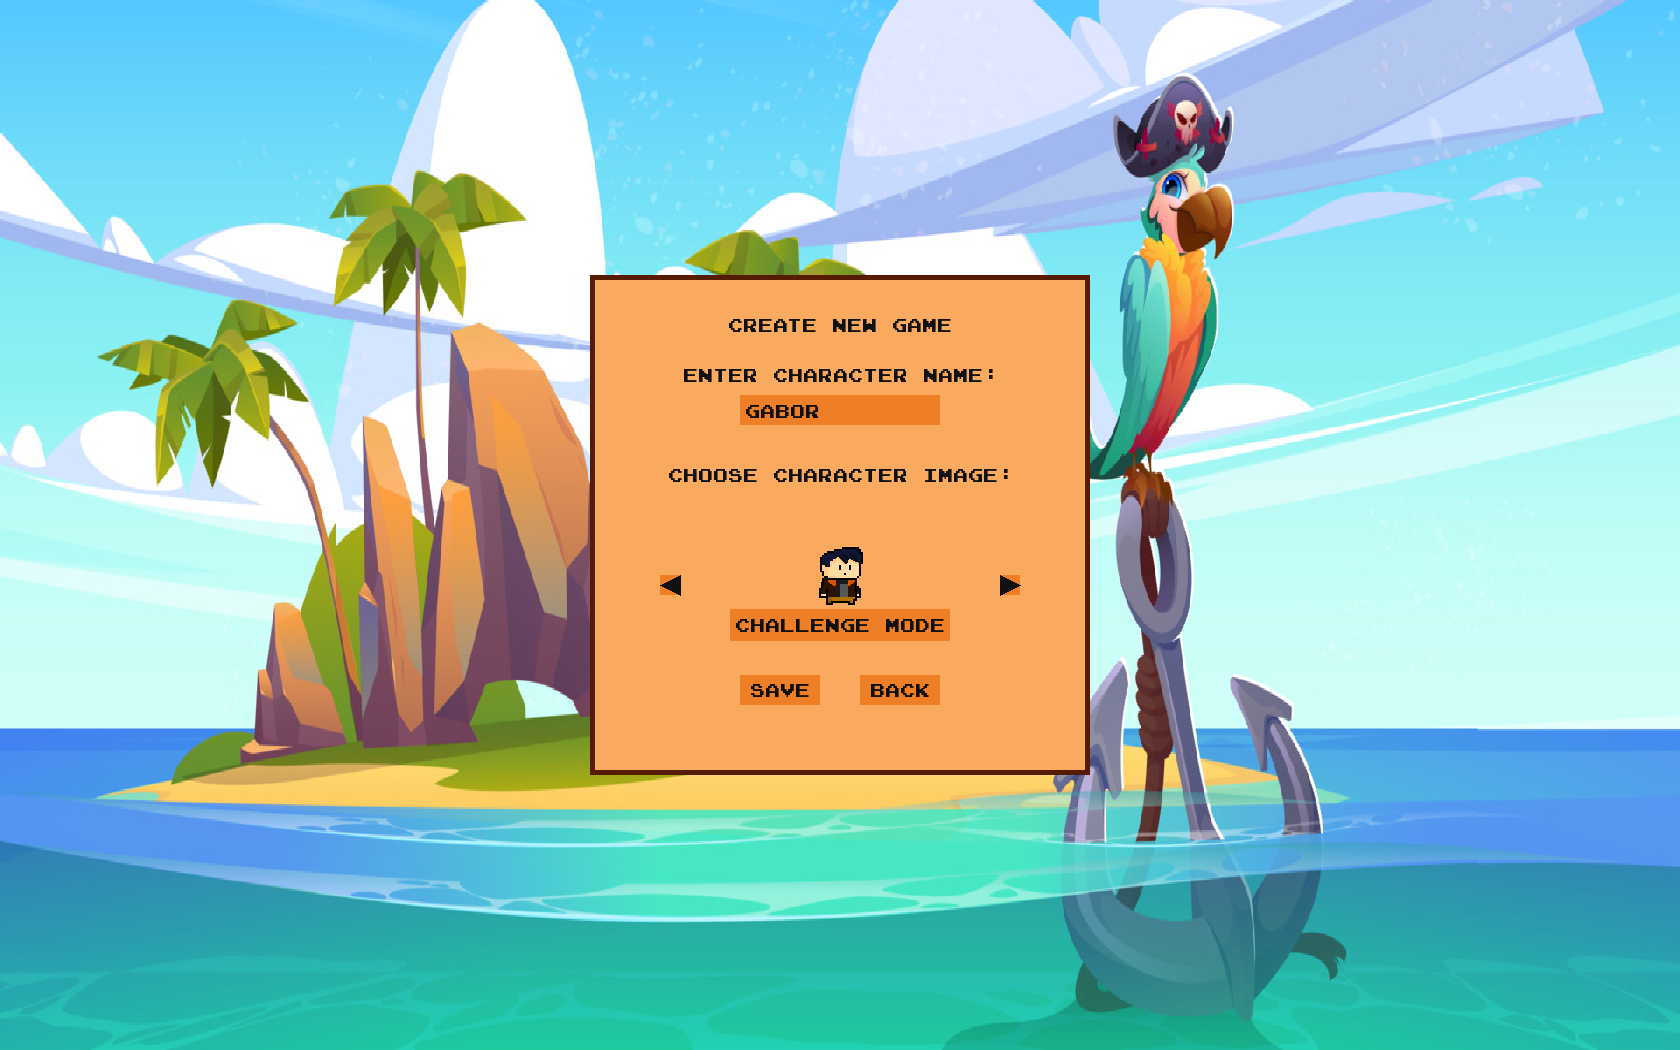
\includegraphics[width=14.0truecm]{images/newgame.png}
    \caption{Új játék létrehozása}
    \label{fig:Új játék létrehozása}
\end{figure}

\subsection{Játékmenet közbeni menü}
\indent \indent Az Esc gomb megnyomásával elérünk egy pillanat állj funkciót, amely egyben egy menüt is megjelenít, ahol a játékosnak lehetősége van a játékállapot mentésére. Illetve folytatni a játékot vagy kilépni az asztalra. (Lásd \ref{fig:Játékmenet közbeni menü})

A pillanat állj funkciót úgy valósítottam meg, hogy az összes játékbeli sprite group, azaz felületi csoport (később bővebben lesz szó ezekről \ref{subsec:Pálya kezelése}) kirajzolására szolgáló függvényt állítom le egy boolean típusú változóval, ezáltal minden játékon belüli elem megáll a legutolsó ismert állapotában, majd a menü bezárása után, amelyet a resume (folytatás) gomb megnyomásával tehet meg a játékos, onnan folytatódnak az események, ahol abbamaradtak.


\begin{figure}[H]
    \centering
    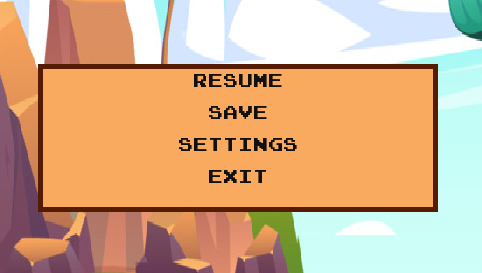
\includegraphics[width=12.0truecm]{images/ingamemenu.png}
    \caption{Játékmenet közbeni menü}
    \label{fig:Játékmenet közbeni menü}
\end{figure}

\subsection{Mentések betöltése}
\indent \indent A játékosnak lehetősége van a korábban elmentett játékállás betöltésére is, amennyiben van ilyen. A betöltés után a játék onnan folytatódik, ahol abbahagyta. Egy lista elrendezésben látja a felhasználó a korábbi mentéseit. Előre rendezi az offline mentéseket a listában, és csak utánuk tölti be az online mentéseket. Egy kattintás után már be is tölti az adott játék állást. Külön nem jelzi, hogy az adott mentés melyik kategóriába tartozik, egyszerűen nem jelennek meg a listában az online mentések, ha nincs bejelentkezve a felhasználó.

\section{Játékmenet kezelése}

\subsection{Main metódus}
\indent \indent Ez az osztály felelős a játék főciklusának végrehajtásáért, ami az egész játék működésének alapját képezi. Amikor a játék elindul, az alkalmazás példányosítja ezt az osztályt.

A \ref{py:főciklus} programkód részletesen bemutatja, hogyan kell megvalósítani ezt a főciklust, amely a játék működéséért felelős. Ebben a kódban kezeljük a játék fő eseményeit, és gondoskodunk arról, hogy minden szükséges műveletet végrehajtsunk a játék folyamán.

Amikor elindul a játék, a bejelentkezési képernyőt találjuk magunkat. A menuenums enum típusban tárolt értékek segítségével dönti el a program, hogy mely állapotot kell megjeleníteni. Itt gondolok, a bejelentkezési képernyőre, főmenüre és annak almenüire, illetve a játékra magára. 

A főciklusban történik, a képrissítés mértékének beállítása a self.clock.tick(Settings.FPS) sorral, az ablak háttérszínének beállítására a self.screen.fill(Settings.WATER\_COLOR) sorral, a játékmenet futtatására a self.game\_handler.run() sorral, és a képernyő frissítésére a pygame.display.update() sorral.

Tehát létfontosságú szerepet játszik abban, hogy a játék működése zökkenőmentes legyen, és a kódban látható példa segítségével könnyen megérthető, hogyan történik mindez.


\begin{python}[caption={Játék főciklusa},label=py:főciklus]
    def run(self):
        while True:
            [...]
            elif self.state == menuenums.GAME:
                if self.game_handler is None:
                    Sounds.play_loop('main')
                    self.game_handler = GameHandler(
                        self.user, self.save_parameters)
                for event in pygame.event.get():
                    if event.type == pygame.QUIT:
                        pygame.quit()
                        sys.exit()
                self.screen.fill(Settings.WATER_COLOR)
                self.game_handler.run()
                pygame.display.update()
                self.clock.tick(Settings.FPS)
\end{python}

\subsection{Játékon belüli felületek} \label{subsec:A játék fő osztálya}
\indent \indent A GameHandler osztály, nagyon fontos szerepet tölt be a játék futása során, több alapvető funkciót kezel. Ez az osztály kezeli a mentéseket erről a későbbiekben \ref{subsec:Játékállapot mentése} szakaszban tárgyalunk majd. 
Kezeli a megjelenített felületeket, értem ezalatt a játékmeneten belüli menüt, ez valósítja meg a pillanat állj funkciót is. Mivel megállítja a LevelHandler (erről a \ref{subsec:Pálya kezelése} szakaszban lesz szó) álltal frissített felületeket. Itt kezelt felület a ranglista funkció, amely a játékmenet megállítása nélkül is látható. Az utolsó általa kezelt felület a karakter fejlesztési panel is, amely a játékos karakterének fejlesztésére szolgál.

\subsection{Játékállapot mentése} \label{subsec:Játékállapot mentése}
\indent \indent A játékállapot elmentését Save gomb megnyomásával lehet elérni. A mentés a játékállapot minden fontosabb elemét eltárolja egy JSON típusú fájlban, ha offline módban játszik a játékos, vagy FastAPI-on \cite{fastapi} keresztül kommunikálva egy MySQL \cite{mysql} adatbázisban, ha online módot választott a felhasználó. 
Minden karakterhez egy mentési lehetőség tartozik, tehát nem lehet egy karakterhez több játékállapotbeli mentést készíteni. Mindig az utolsó mentés kerül felülírásra, ha a játékos új mentést készít. Ebből következik, hogy a játékosnak mentéskor nincs lehetősége rálátni a korábbi mentéseire, csak a betöltési menüben, ahol a játékos kiválaszthatja a korábbi mentéseit.

\subsection{Pálya kezelése} \label{subsec:Pálya kezelése}
\indent \indent Levelhandler a másik nagyon lényeges osztály, ez a GameHandler-ben kerül példányosításra. Feladata a világok, a kamera, entitások létrehozása és kezelése ellentétben a GameHandler osztállyal (Lásd \ref{subsec:A játék fő osztálya}) amely feladata a játékon belül elérhető funkciók kezelése, értem ezalatt a menük megjelenítését, mentést vagy a pálya futtatását. 
Ezeket a különböző felületeket Sprite Group-okba szervezve kezeli, így könnyen tudja őket elérni és frissíteni. Ezeket a csoportokat a Tiled-ben létrehozott rétegek alapján határozza meg, milyen felület milyen jellemzőkkel fog rendelkezni.
Legfontosabb ezek a sprite csoportok közül talán a Visible Sprite csoport, amely a játékos által látható felületeket tartalmazza. A kamera ezeket rendereli ki úgy, hogy ezeket a csempéket y tengely szerint rendezi és úgy jeleníti meg, hiszen, ha az alapértelmezett x tengelyen haladna végig a kirajzolási funkció, akkor nem lehetne elérni hamis 3D hatást. Jelenleg, ha a karakter egy fa ``felett'' tartózkodik azt félig rá rajzolja ki ezáltal elérve mintha mögötte bújkálna a karakter, de ez minden elérhető felületre igaz. Maradva az előző példánál, ez x tegnely szerinti rendezésben esetében úgy nézne ki, hogy a karakter a fa baloldalánál állva a fa mögött helyezkedne el, azaz a karaktert kitakarná, ameddig a jobb oldalán a karakter lenne az előtérben. 
Megtalálható még obstacle (akadály), attack (támadó), és attackable (támadható) felület csoportok is, amelyek a játékmenet során fontos szerepet játszanak, különböző mechanikák végrehajtásánál. Az obstacle csoportba \ref{fig:Tiled} ábrán piros körvonalú rétegen szereplő csempék kapták, amelyek szerepe, hogy az ütközésvizsgálat ebbe a csoportba tartozó csempéket veszi figyelembe. Az attack csoportba a játékos által irányított karakter támadó felületei kerültek azaz a fegyverek, hiszen ezeket nagyon rövid ideig kell megjeleníteni ezután törölni azokat. Az attackable csoport szorosan kapcsolódik az utóbb említett csoporthoz. Ide tartozik az összes olyan felület, amelyekkel a fegyverek interakcióba kerülhetnek. Ebbe a csoportba tartoznak például a szörnyek, de a fűcsomók is amelyeket a játékos ki tud ütni a fegyverével. 

\subsection{Világ és barlangok} \label{subsec:Világ és barlangok}

\indent \indent A játékos amikor létrehoz egy új karaktert, vagy beölt egyet akkor egy világban fogja találni magát. Ez a világ a fő pályarész, itt helyezkedik el minden kulcsontosságú helyszín és karakterek. Illetve a játék során ellehet látogatni egy barlangba ami egy nagyságrendileg kisebb terület, amelyből több is létezhet egy világban.
 A world és a dungeon osztály közös szülő osztályból származnak le, ez azért fontos, hogy a különböző világokat könnyen tudjam kezelni
 és különböző tulajdonságokat adni nekik. Ebben az osztályban a minden világra vonatkozó lehetőségeket kezelem, ilyen például
  az effekteket lejátszó AnimationPlayer osztályom származtatása, mert azt elég egyszer definiálni és meghívni ott, ahol szükséges, ahelyett,
   hogy minden világnak lenne egy külön példánya. Továbbá ilyen opció a térképmegnyitás, és az azzal kapcsolatos összes funkció,
    például, hogy hol található a következő küldést adó nem játékos karakter. A játék története jelenleg teljesen lineáris,
     tehát egy adott sorrendben történhet csak a küldetések teljesítése. Ez az osztály kezeli szörnyek legyőzése által elejtett, hátrahagyott tárgyakat, ilyen tárgyak a tapasztalati pont és az aranypénz.
       Ezeket a tárgyakat a játékos össze tudja gyűjteni, és a későbbiekben fel tudja használni.  

\subsubsection{Pálya generáláshoz szükséges adatok} \label {subsec:Pálya generáláshoz szükséges adatok}

\indent \indent Említettem a korábbi fejezetben, a pálya megtervezését a \textbf{Tiled}-el végeztem. (Lásd \ref{subsec:Tiled}) 
Első megközelítésemben CSV (vesszővel elválaszott értékek) fájl formátumba mentettem ki a tervezőben létrehozott rétegeket. Egy ilyen dokumentum úgy néz ki, hogy ahova nem helyeztem le a tervezőben objektumot, ott '-1' érték szerepel, ellentétben ahol van érték, ott a Tiled-ben betöltött és feldarabolt csempekészlet azonosító számai kerültek a dokumentumba. Ezt úgy kell elképzelni, mint egy nagy mátrixot. Az utolsó pillanatokig ezt a megközelítést alkalmaztam, mert ha már kész volt és működött, miért változtattam volna rajta. Végül mégis visszatértem erre a kérdéskörre és készítettem az alább olvasható kis egyszerű átalakító szkriptet. (Lásd \ref{py:csvtodict} programkód) Ennek funkciója, a sok felesleges '-1' értéket kiszűrni, hogy a program futása közben ne kelljen a betöltésnél rengeteg felesleges összehasonlítást végezni. Ezt úgy oldottam meg, hogy készítettem python dictionary-t a csempe azonosító számából, illetve annak a .CSV mátrixban elhelyezkedő koordinátáiról. (Lásd \ref{py:átalakított struktúra} programkód)


\begin{python}[caption={CSV formátum dictionary formátumra konvertálása},label=py:csvtodict]
    import csv
    import json
    
    csv_file = "new_map\MSmap._dungeonentrance.csv"
    map_data = []
    
    with open(csv_file, newline='') as csvfile:
        csv_reader = csv.reader(csvfile)
    
        for i, row in enumerate(csv_reader):
            for j, value in enumerate(row):
    
                value = int(value)
                if value != -1:
                    map_data.append({"i": i, "j": j, "value": value})
    
    python_file = "world_dungeonentrance"
    
    with open(python_file, 'w') as pyfile:
        pyfile.write("map_data = ")
        json.dump(map_data, pyfile, indent=4)
    
    print(f"Dictionary saved to {python_file}")
    
\end{python}


Készítettem egy kis függvényt, a pálya létrehozásának idejének lemérésére. Ez azért volt fontos, hogy megtudjam határozni, hogy a szótár használata jobb megoldás-e, mint a CSV fájl. A két megoldás esetében a következő eredményeket kaptam:

\begin{itemize}
    
    \item Python dictionary esetében:
    \begin{verbatim}
        Futási idő: 108.64 ms
    \end{verbatim}
    \item Comma-Separated Values (CSV) esetében:
    \begin{verbatim}
        Futási idő: 879.92 ms
    \end{verbatim}
\end{itemize}
    
\indent \indent Tehát elmondható, hogy ez a változtatás jelentősen felgyorsította a pálya létrehozását, ezáltal a játék betöltési ideje is csökkent.



\begin{python}[caption={Minta az átalakított struktúrára
    }, label=py:átalakított struktúra]
    {
        "i": 3,
        "j": 41,
        "value": 125
    },
\end{python}

\subsubsection{Pálya generálás}

\indent \indent A korábban (lásd \ref{subsec:Tervezés}) megtervezett és exportált majd feldolgozott (Lásd \ref{subsec:Pálya generáláshoz szükséges adatok}) pályaadatok megjelenítését több lépésben valósítottam meg. Először is a képeket be kell tudnom olvasni, ezt az os \cite{Python-os} könyvtár walk függvényének segítségével oldottam meg.
 Miután sikerült bejárni a mappát, előállította az egyes képekhez vezető útvonalat, ezután a pygame.image.load() függvényével betölti a képeket. A képeket entitás esetében képkockánként, míg a pálya esetében mozaik-kockák formájában tároltam.
  Ezt követően a képeket egy listába helyeztem, amelyet később fel tudok használni a kirajzoláshoz.
   Másik ilyen fontos lépés a pálya rétegek beolvasása, amelyet a korábban említett dictionary segítségével valósítottam meg.
    Ezután egy ciklusban végig iterálva a dictionary-n, a képek listájából kiválasztotta a megfelelő képet, és a megfelelő koordinátákat,
     amelyeket segítségével példányosítom a Tile osztályt, később ennek segítségével végzi el a kirajzolást.
      Mivel a szótárak között szerepel az entitásokra vonatkozó réteg is, ezért azokat is az előbb említett iterációban kezeltem,
       és példányosítottam a hozzájuk tartozó osztályokat, azonosító alapján szűrve.

\subsection{Entitások}
\indent \indent Ez az osztály egy szülő osztály amit az Enemy, NPC és Player osztályok használnak. A szülő osztály azt jelenti, hogy ebből származnak le más osztályok és felhasználják minden tulajdonságát, illetve metódusait is.  

Három fontos metódussal rendelkezik, az egyik a mozgás kezelése. A mozgást a move függvény segítségével hajtja végre, amelynek a lényege, hogy az entitás rendelkezik egy irány változóval, ami tárolja, hogy merre néz (ez lehet fel, le, jobbra, balra), és ezeknek az irányoknak a vektorának normalizálásával és a paraméterként megkapott sebesség értékkel meghatározza a következő pozícióját az entitásnak. A normalizás azért fontos, hogy átlós mozgás esetén ne mozogjon az adott karakter sokkal gyorsabban. A vektor egységesítéséhez, normalizálásához a vektor minden egyes komponensét el kell osztani annak hosszával, ezzel elérve, hogy a vektor iránya ne változzon, csak a hossza legyen 1. A pozíció módosítás az egyed hitbox-ára vonatkozik, azaz arra a dobozra, amely az entitást körülveszi. Azért a hitbox-ot kell mozgatni, mert a szörnyek és karakterek képei a hitboxra vannak igazítva. Ez azért fontos, mert így megelőzhető az olyan hibák előfordulása, amit a hitbox és a kép közötti eltérés okozhatna. Ilyen szinkrinizációs hiba, például lövöldözős játékok esetében szokott látványosan előfordulni, hogy egy bizonyos testrész hitbox-a nem ott helyezkedik el ahol a grafika, és a játékosok miközben látják, hogy eltalálják az ellenfelet, mégsem történik sebzés.

A másik egy szinusz függvény alapján ad vissza 0-255 értéket, ez arra szolgál, hogy az elszenvedett sebzés után villogó effekt játszódjon le az adott entitáson, ezzel jelezve meddig sebezhetetlen. A harmadik metódus az ütközés érzékelésre, kezelésére szolgál.

Az ütközés érzékelés lényegében úgy működik, hogy nézzük az entitás mozgási irányát, hogy függőlegesen, vagy vízszintesen közlekedik, és az adott iránytól függően vizsgáljuk, hogy az entitás fizikai kiterjedése (későbbiekben hitbox), esetemben egy grafika nagyságú téglalap ütközik-e valamelyik korábban említett obstacle, akadály csoport csempével. Ha igen, akkor az entitás irány szerinti hitbox határát az akadály ellenkező irányű hitbox határához igazítjuk, így megakadályozva az áthaladást, de nem letiltva a többi irányba való mozgást. (Lásd \ref{fig:Ütközés kezelése} ábra, és \ref{py:Ütközés kezelés} programkód)




\begin{python}[caption={Ütközés kezelése},label=py:Ütközés kezelés]
def collision(self, direction):
    #horizontalis mozgas
    if direction == 'horizontal':
        for sprite in self.obstacle_sprites:
            if sprite.hitbox.colliderect(self.hitbox):
                if self.direction.x > 0:
                # jobbra mozgas
                    self.hitbox.right = sprite.hitbox.left
                if self.direction.x < 0:
                # balra mozgas
                    self.hitbox.left = sprite.hitbox.right                   
    #vertikalis mozgas
    if direction == 'vertical':
        for sprite in self.obstacle_sprites:
            if sprite.hitbox.colliderect(self.hitbox):
                    if self.direction.y > 0:
                        # lefele mozgas
                        self.hitbox.bottom = sprite.hitbox.top
                        if self.direction.y < 0:
                        # felfele mozgas
                        self.hitbox.top = sprite.hitbox.bottom
                    \end{python} 


                    \begin{figure}[H]
                        \centering
                        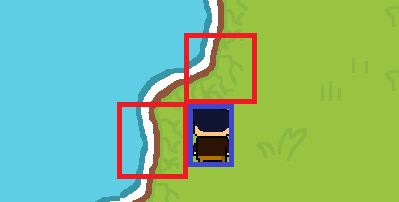
\includegraphics[width=15.0truecm]{images/collision.png}
                        \caption{Ütközés kezelése}
                        \label{fig:Ütközés kezelése}
                    \end{figure}
                    
                    
\subsection{Játékos karaktere}
\indent \indent Ez az osztály a játékos karakterét valósítja meg, amely a játék során irányítható. A játékos karaktere egy entitás, így örökli az entitás osztály összes tulajdonságát és metódusát.

Az osztály inicializálása során számos fontos adatot tárol, például a játékos nevét, karakterének azonosítóját és kezdeti pozícióját. Ezek az adatok meghatározzák a karakter kezdeti állapotát a játékban.

A karakter mozgását és irányítását az osztály input metódusa kezeli. Ennek segítségével az osztály figyeli, hogy milyen billentyűk vannak lenyomva, és ennek megfelelően mozgatja a karaktert a játékban. A játékos karakter képes balra, jobbra, felfelé és lefelé mozogni a megfelelő billentyűk lenyomásával.

A karakter sebessége és energiaszintje dinamikusan változik a játék során. Például a karakter gyorsabban mozoghat, ha lenyomja a ``SHIFT'' billentyűt, és az energia szintje csökken mindeközben. Az energia idővel regenerálódik, ami lehetővé teszi, hogy tovább használhassa a gyors futás funkciót.

A játékos karakter képes támadni is, és az attack metódus meghívásával hozza létre a támadást. A támadásokat az osztály figyeli, és számítja ki a támadások között eltelt időt, hogy ne lehessen túl gyorsan ütni a fegyverekkel.

A karakter fegyvere is dinamikusan változik, és a játékos lehetőséget kap a fegyver cseréjére a játék során.

A karakternek vannak életpontjai és energia szintje, amelyek meghatározzák a túlélését a játékban. Amennyiben az életpontja nullára csökken, a karakter meghal, de van lehetőség a visszatérésre vagy újrakezdésre a játékban, attól függően, hogy milyen a játék nehézségi szintje.

A karakter számos egyéb tulajdonsággal és képességgel rendelkezik, például tapasztalati pontokkal, megszerzett arany mennyiségével és teljesített küldetésekkel. Ezek a tényezők befolyásolják a játékmenetet és a karakter fejlődését.

Az osztály továbbá lehetővé teszi a karakternek, hogy tárgyakat használjon és rendelkezzen egy táskával. A játékos képes tárgyakat váltani és használni a játék során, ami további taktikai elemet ad a játékhoz.

Összességében ez az osztály kulcsfontosságú a játékos karakter kezelésében és irányításában, lehetővé téve a játékosnak, hogy részt vegyen a játék világában és kihívásokkal nézzen szembe a karaktere fejlesztése során.

\subsection{Fegyverek}

\indent \indent A különböző fegyverek (Lásd \ref{fig:A játékban megtalálható fegyverek} ábra) használata szintén egy elengedhetetlen része a játéknak. A fegyvereket a játékos karaktere használja a szörnyek elleni harc során. Közlehraci fegyvereket valósítottam meg, a kard, a lándzsa, a kétkezes kard és a kétkezes lándzsa. Ezek a fegyverek különböző támadási távolsággal és sebzéssel rendelkeznek, előkészítettem a támadási sebesség megvalósítását is, de az végül nem került be a játékba, mert szerintem rontotta volna a játékélményt.

Ezen harcolásra szolgáló eszközök kirajzolása a támadás gomb lenyomása után történik a Weapon osztály példányosításával. Ez az osztály a játékos karaktere által kezében tartott fegyvert rajzolja ki a képernyőre. Mivel fontosnak tartottam, hogy mozgás közben is lehessen támadni, illetve legyen egy csapás/suhintás animáció, ezért egy frissítés funkciót vezettem be, amely mindig a játékos karakterének legutóbbi helyzetét, és irányát vizsgálja, majd ezekre az adatokra alapozva frissíti a már létrehozott képet. A csapás animációt mind a négy irányban külön-külön kellett megtervezni, mert a fegyverek nem egyformán néznek ki minden irányból. Szinusz függvény segítségével valósítottam meg a megjelenített fegyver forgatását egy amplitúdó értékkel, amely a fegyver típusától függően változhat.

Ahogyan a többi látható objektum, ezek a fegyverek is a visible sprite csoport része, viszont egyben az attack\_sprites csoport része is, amely segít megkülönböztetni a többi felülettől a fegyvereket, ezáltal támogatva a támadási logika megvalósítását. A támadási logika egy metódus, amely ezen az attack\_sprites csoporton végig iterál, és vizsgálja az attackable\_sprites felületekkel való ütközést, amelyeket olyan entitások kaphatnak, amelyekkel a játékos meg tud küzdeni a játék során. Legyen az egy szörny vagy akár egy kiüthető fűcsomó. 

\begin{figure}[H]
    \centering
    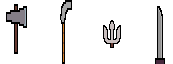
\includegraphics[width=15.5truecm]{images/weapons.png}
    \caption{A játékban megtalálható fegyverek}
    \label{fig:A játékban megtalálható fegyverek}
\end{figure}


\subsection{Ellenségek, szörnyek}

\indent \indent Az ellenségek a játékban a küldetések után talán a legfontosabb mechanikái a játéknak, mert a velük való harc kiemelt szerepet kap a történet során.
Az Enemy osztálynak is az Entity a szülő osztálya, ez biztosítja, hogy mozoghassanak a szörnyek. Szerettem volna, hogy az ellenségeket különböző tulajdonságokkal tudjam felruházni, de mégis egységesen tudjam kezelni. Például a sebesség, életerő, támadási sebesség, támadások hangjai. Ezeket a tulajdonságokat a settings statikus osztály monster\_data dictionary-jében tárolom és olvasom be. És a szörnyek típúsa alapján ezeket a tulajdonságokat beállítom az adott szörny példányosításakor.

A szörnyek mozgását úgy valósítottam meg, hogy ha a játékos egy adott sugáron belül ér a szörnyhöz képest, ez az úgynevezett érzékelési sugár, akkor kiszámolom vektorokkal a játékos távolságát, és ha a távolság nagyobb, mint 0, azaz nem egy helyen állnak, akkor meghatározom az irányt a két vektor különbségének normalizálásával. A távolság érték azért fontos, hogy megállíptsa mikor ér a játékos karaktere a szörnyhöz támadási távolságon belülre. Az irány érték pedig a szörny mozgatásához szükséges.

Három különböző státusszal rendelkezhet egy ellenség. Támadási státuszt kap, ha támadási sugáron belül tartózkodik a játékos karaktere, és ha egy bizonyos idő eltelt az előző támadás óta. Mozgás státuszt kap, ha a játékos karaktere a szörny érzékelési sugarán belül van, de nem támadási sugáron belül. Ha a játékos karaktere nincs az érzékelési sugarán belül, akkor pedig nyugalmi státuszt kap. Ezek a státuszok határozzák meg a szörnyek viselkedését és a megjelenített grafikát is a játék során.


\subsection{Zsákmányolás}


\begin{figure}[H]
    \centering
    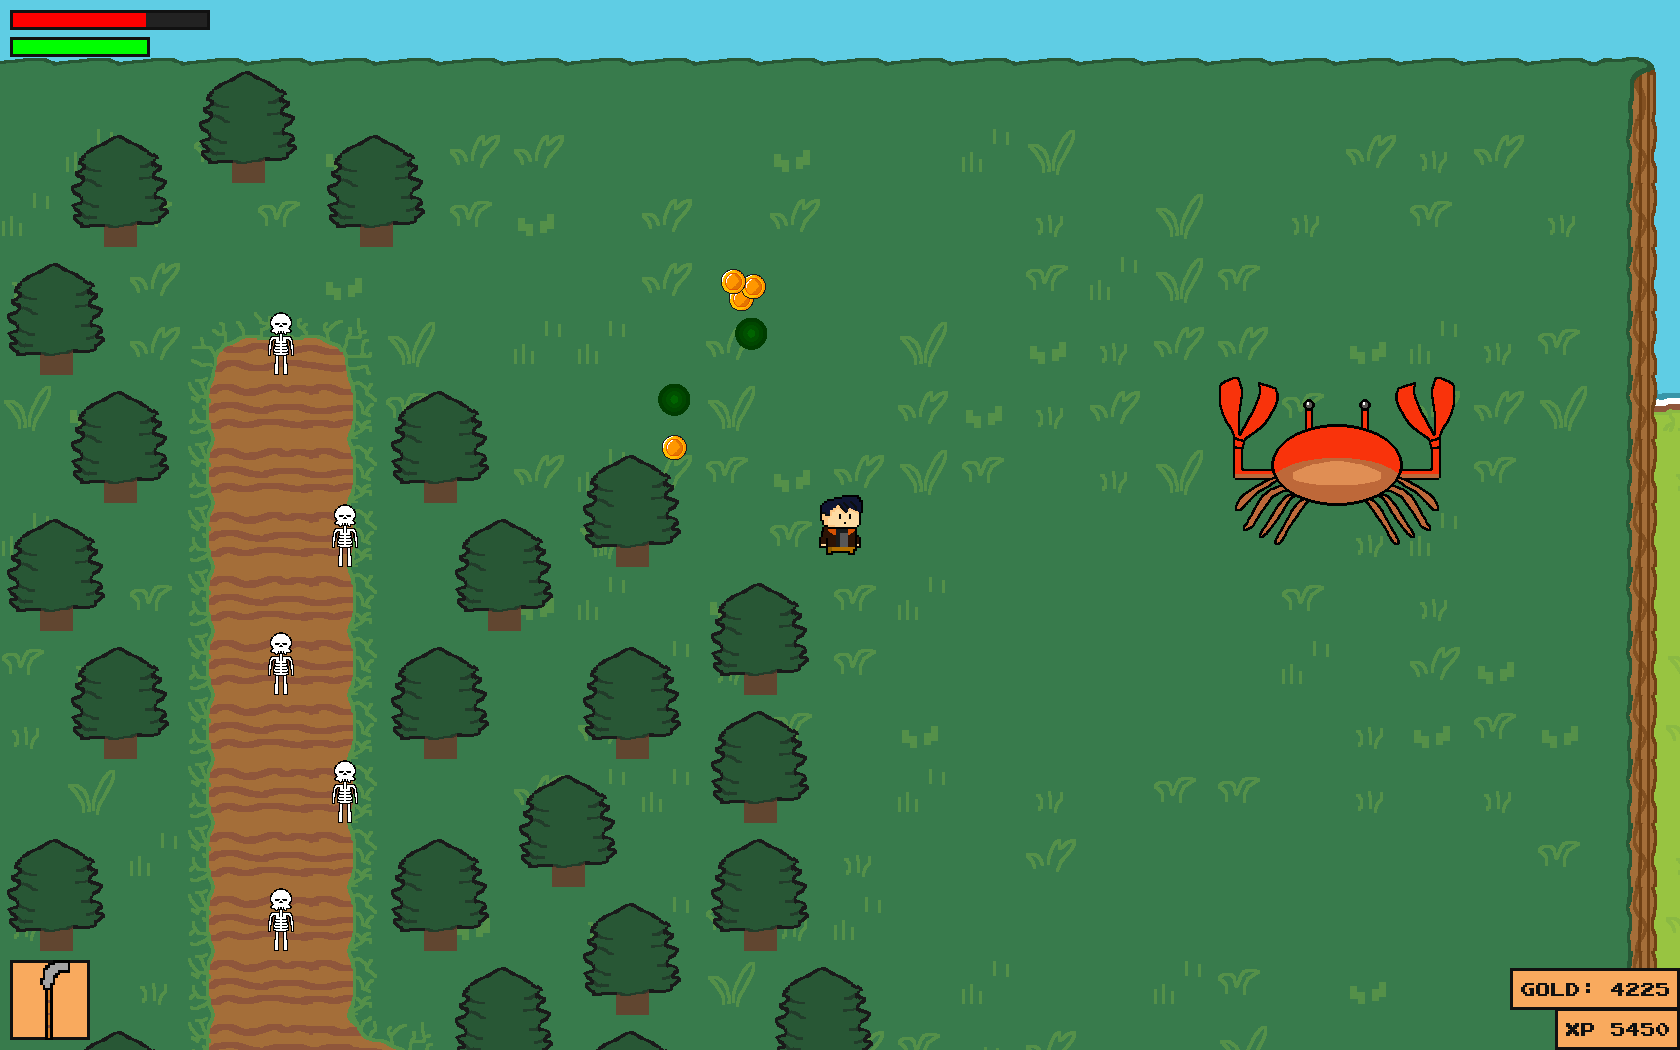
\includegraphics[width=15.5truecm]{images/loots.png}
    \caption{Zsákmányolás funkció}
    \label{fig:Zsákmányolás funkció}
\end{figure}

\subsection{Nem a játékos álltal vezértelt karakterek}
\indent \indent Nem játékos által vezértelt karakterek, azaz NPC-k egy kalandjáték során elengedhetetlen részei a történetnek és a játékmenetnek. A szörnyek sem a játékos által vezérelt karakterek, de a játékokban az NPC megjelölést általában az egyéb, békés szerepet betöltő karaktereket hívjuk. Ahogy az szörnyek és a játékos is az Entity osztályból származik le úgy az NPC is, mert adott esetben szükség lehet mozgatásra és ütközés érzékelésre. Azonban a legtöbb esetben a játékos karaktere nem tudja megölni ezeket az entitásokat, mert a történet során szükség van rájuk. Ezért a játékos karaktere nem tud ütközni velük, és a szörnyekkel ellentétben nem tudnak támadni.


\subsection{Küldetést adó karakterek}

\indent \indent A játékom egyik legfontosabb mechanikája a küldetés rendszer, mert ezen alapszik az előrehaladás, illetve a challange játékmódnál az újraindítás is a küldetések teljesítését érzékelve valósul meg. 

A Questgiver NPC (küldetést adó karakter) típust a World osztályban példányosítom, (Lásd \ref{subsec:Világ és barlangok}) és
 a példányok osztályváltozóinak inicializálásakor olvassa be a saját id-jéhez tartozó küldetéseket a Settings osztály npc\_data dictionary-jéből.
  Majd ezt követően a World osztály létrehoz a Player osztályból is egy példányt,
   amely egészen a LevelHandler osztálytól (amit már korábban említettem \ref{subsec:Pálya kezelése}) kap
    paraméterként egy questgivers\_quest\_setup függvényt amely egy trigger (aktiváló esemény) után vizsgálja,
     hogy a játékos álltal már teljesített küldetés szerepel\-e még Questgivernél. Igaz visszatérési érték esetén kitörli azt,
      ezáltal elkerülhető a küldetés ismétlődése. Küldetést nem lehet kihagyni, mindegyiket sorban kell teljesíteni,
       ahogy a történet halad előre. Elutasítás esetén a küldetés nem törlődik, csak a dialógus ablak bezáródik és a játékban a linearitása miatt nem lehet tovább haladni.

Az questgiver típusú NPC-k képesek egy előre megírt dialógus megjelenítésére (Lásd \ref{fig:Dialógus rendszer} ábra), amelyben a játékos választhat két lehetőség közül, amelyek a küldetés elfogadása vagy elutasítása. A választás megerősítése történhet a kurzornak a gomb felé mozgatásával, ezután egy kattintással, vagy a billentyűzet segítségével egyaránt. A dialógus ablak megnyitásához szükséges a játékos karakteréhez viszonyított távolság érzékelése, mert egy beszélgetés során közel kell állni a kommunikációban résztvevő többi szereplőhöz, ezt hasonló módon vizsgálom, mint ahogy a szörnyek esetében az érzékelési távolságot vizsgáltam. Illetve dialógus megjelenítéséhez még szükséges, hogy az adott NPC rendelkezzen a soron következő küldetés azonosítójával is.   

\begin{figure}[H]
    \centering
    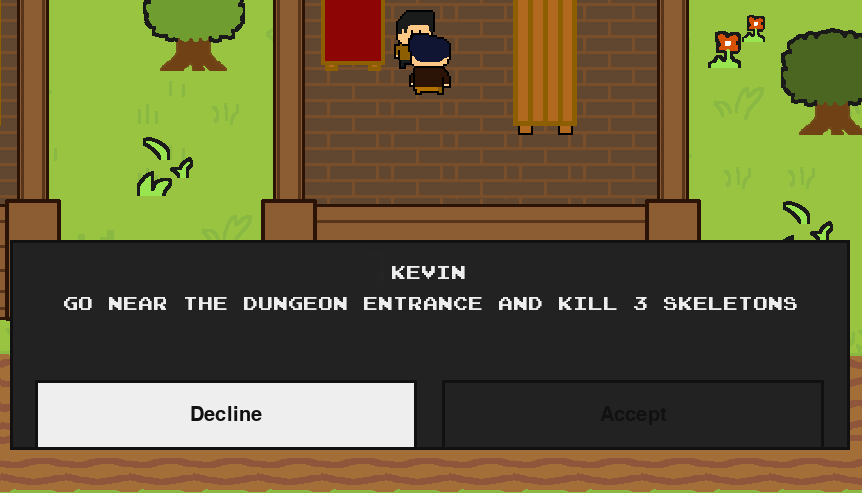
\includegraphics[width=10.0truecm]{images/dialogue.png}
    \caption{Dialógus}
    \label{fig:Dialógus rendszer}
\end{figure}

\subsection{Kereskedő karakter}

\indent \indent Egy kalandjátékban az előrehaladás mellett fontos, hogy a nehezen megszerzett tárgyakkal,
 esetünkben az arannyal lehessen mit kezdeni, ezért egy Merchant NPC (kereskedő karakter) típus létrehozását láttam a legjobb ötletnek,
  mert rengeteg különböző módon fel lehet őket használni. 

Egyenlőre csak bájital árusításra szolgáló merchant van a játékban (élet visszatöltő, energiát növelő, sebzést növelő bájitalok árusítására szolgál).
   Ahogyan a Questgivernél, itt is a távolságvizsgálat alapján és egy gomb lenyomására történik a vásárlásra szolgáló ablak megjelenítése (Lásd \ref{fig:Merchant} ábra).
     A vásárlás során a játékos karakterének az egyenlege/arany mennyisége csökken, és a vásárolt tárgyak a hátizsákjába kerülnek.

Azt, hogy milyen tárgyakat adhat el egy bizonyos merchant, azt a Settings osztályból egy dictionary-ben tárolt azonosítók beolvasása befolyásolja.
 Illetve a Settings osztály tartalmaz egy Items dictionary-t is, amelyben a tárgyakra vonatkozó adatokat tárolom.
  Ilyen adatok például a tárgy neve, típusa, ára, hatása és annak mértéke (Például mennyi plusz erő-t ad a tárgy),
   és időtartama és a grafikának az elérési útvonala.  

\begin{figure}[H]
    \centering
    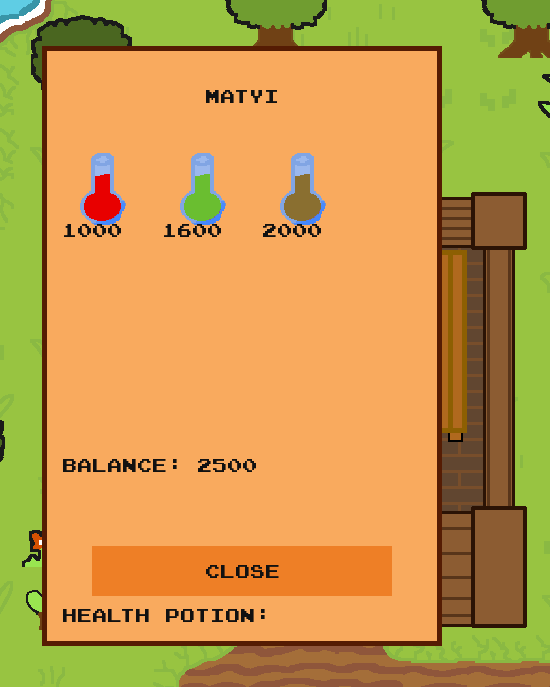
\includegraphics[width=9.0truecm]{images/merchant.png}
    \caption{Kereskedő karakter}
    \label{fig:Merchant}
\end{figure}


\subsection{Táska rendszer}

\indent \indent A Quickslot azaz táska rendszer, fontos szerepet kap a játék folyamán, mert a merchanttól megvásárolt tárgyak ebbe a táskába kerülnek bele. A játékos ezeket tudja felhasználni amikor szükségét érzi, akár harc közben is.

Öt szabad férőhellyel rendelkezik a táska, ezért jól meg kell válogatni, melyek azok a fontos tárgyak, amelyeket oda szeretne helyezni a játékos. Első nekifutásra egy futószalag szerű működést képzeltem el a táska rendszernek, amelyet azért gondoltam jó ötletnek, mert a megvalósítása egyszerű volt, mert megszerzett tárgyak időrendben kerültek bele a táskába. Viszont felmerült a probléma, hogy ha más sorrendben esik kézre a felhasználónak, vagy nincs helye, akkor mit tud tenni. Ezért úgy döntöttem, hogy jobb megoldás lenne, ha az azonos tárgyakkat össze lehetne húzni egy férőhelyre, ezáltal kényelmesebbé válna a használata a táskának. Megtartottam a futószalag szerű megoldást, viszont kiegészült a tárgy összevonással, amelyet egy számláló bevezetésével oldottam meg, amely jelzi a felhasználónak, hogy még mennyi található nála abból az adott tárgy típúsból. (Lásd \ref{fig:Táska rendszer} ábra)

\begin{figure}[H]
    \centering
    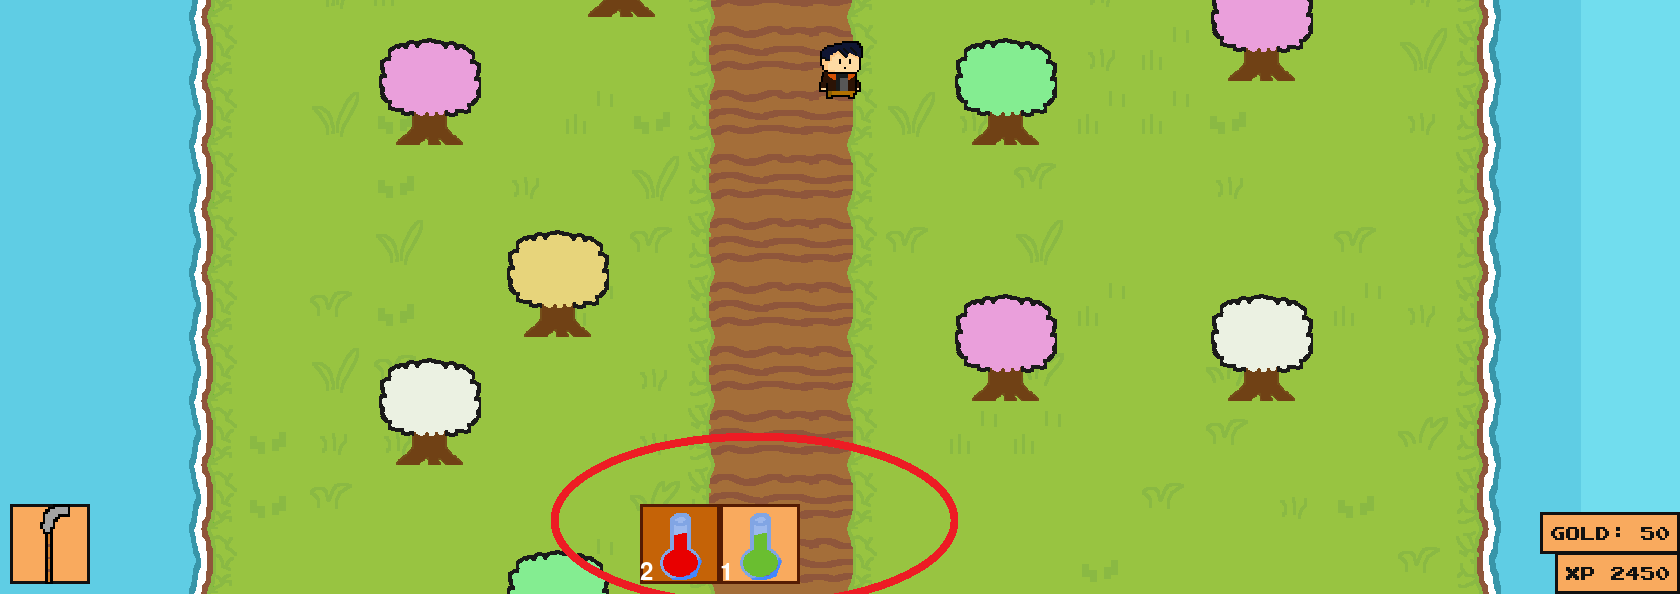
\includegraphics[width=15.5truecm]{images/inventory.png}
    \caption{Táska rendszer}
    \label{fig:Táska rendszer}
\end{figure}


\section{Adatbázis használata a programban}

\indent \indent Az online mentés kezeléséhez, illetve a játékban való regisztrációhoz és bejelentkezéshez szükség volt egy backend megvalósítására, azaz egy alkalmazásra, amely kommunikációt végez a MySQL \cite{mysql} adatbázissal. Az adatbázis struktúrát a MySQL Workbench \cite{mysql-workbench} asztali alkalmazásban építettem fel, eddig az általam használt alkalmazások küzül ez volt ami felhasználóbarát módon volt megvalósítva.  A kommunikációt a FastAPI \cite{fastapi} nevű python könyvtár segítségével valósítottam meg. A FastAPI egy modern, gyors, könnyű keretrendszer a microservice-ekhez talán a legjobb választás python programozási nyelv esetében.

Az adatokat különböző requestek és a megfelelő endpointok segítségével tudjuk elérni, vagy adott esetben felvinni, frissíteni.
 A FastAPI érzékeli, hogy egy kérés érkezett a rendszerbe, és ha az adott kérés teljesíthető,
  akkor az esetemben megkezdi a kommunikációt a mysql adatbázissal és a visszakapott adatokat BaseModell \cite{basemodell} típusú objektumokba tölti,
   amelyekek a Pydantic \cite{pydantic} könyvtárnak köszönhetőek. Ez a modell azért fontos, mert validálja,
    hogy a kérésben szereplő adatok megfelelnek-e a megadott adatstruktúrának.
     Miután a validálás is sikeresen lezajlott, a FastAPI visszaküldi a végpont kérésre a megfelelő választ.

